\section{Design Theory for Relational Databases}
    
  Okay, we know all that is needed to define a database, but not how to work practically well with it yet. Given some set of data or some structure, we must find an optimal way to store it, within either one or multiple relations. How should we do this? The first step is to categorize the potential problems. 

\subsection{Anomalies and Decomposition}
  
  \begin{definition}[Anomaly]
    Beginners often try to cram too much into a relation, resulting in \textbf{anomalies} of three forms. 
    \begin{enumerate}
      \item \textit{Redundancies}. Information repeated unnecessarily in several tuples. 
      \item \textit{Updates}. Updating information in one tuple can leave the same information unchanged in another (which violates referential integrity). 
      \item \textit{Deletion}. If a set of values becomes empty, we may lose other information as a side effect (another violation of referential integrity). 
    \end{enumerate}
  \end{definition}

  \begin{example}[Redundancies]
    Let's try to see where these anomalies came from. Consider a non-trivial FD $\mathbf{a} \mapsto \mathbf{b}$ where $\mathbf{a}$ is not a superkey. Since $\mathbf{a}$ is not a superkey, there are attributes, say $\mathbf{c}$ that are not functionally determined by $\mathbf{a}$. Therefore, there are multiple combinations of $\mathbf{a, b, c}$ which have the same $\mathbf{a, b}$ but not $\mathbf{c}$, leading to redundancy. 

    \begin{table}[H]
      \centering
      \begin{tabular}{|c|c|c|}
        \hline
        \textbf{a} & \textbf{b} & \textbf{c} \\
        \hline
        $x$ & $y$ & $z_1$ \\ 
        $\vdots$ & $\vdots$ & $\vdots$ \\ 
        $x$ & $y$ & $z_{100}$ \\
        \hline
      \end{tabular}
      \caption{Redundant information in \textbf{a} and \textbf{b} attributes. }
      \label{tab:redundant}
    \end{table}
    If $T_{\mathbf{a}}, T_{\mathbf{b}}$ are both 4-byte integers, we have just wasted 400 bytes of space. It seems that most of the redundancy comes from using $a$ and $b$ too many times. If we had two relations $R$ and $S$. 
  \end{example}

  To eliminate these anomalies, we want to \textbf{decompose} relations, which involve splitting $R$ into two new relations $R_1, R_2$. 

  \begin{definition}[Decomposition]
    Given relation with schema $R(\mathbf{A})$, we can decompose $R$ into two relations $R_1 (\mathbf{A}_1)$ and $R_2 (\mathbf{A}_2)$ such that 
    \begin{enumerate}
      \item $\mathbf{A} = \mathbf{A}_1 \cup \mathbf{A}_2$ (not necessarily disjoint)
      \item $R_1 = \pi_{\mathbf{A}_1} (R)$
      \item $R_2 = \pi_{\mathbf{A}_2} (R)$
    \end{enumerate}
    There are two types of decomposition: 
    \begin{enumerate}
      \item \textbf{lossy} decomposition of $R$ to $R_1, R_2$ means that joining $R_1, R_2$ does not give us $R$. 
      \item \textbf{lossless} decomposition indeed gives us back $R$. 
    \end{enumerate}
  \end{definition}

  \begin{theorem}[Decomposition]
    Any decomposition $R_1, R_2$ of $R$ satisfies 
    \begin{equation}
      R \subset R_1 \bowtie R_2
    \end{equation}
  \end{theorem} 
  \begin{proof}
    If $R_1.\mathbf{A} \cap R_2.\mathbf{A} = \emptyset$, then $R \subset R_1 \times R_2$ for sure. If there is some overlap, then given some $r \in R$, we will be able to find $r_1 \in R_1$ and $r_2 \in R_2$, and they will definitely join in their overlapping attribute, giving $R$. 
  \end{proof}

  Therefore, we should be worried about if our decomposition will create \textit{new} tuples since it will never delete relevant ones.

  \begin{example}[Lossy and Lossless Decomposition]
    Consider the relation 
    \begin{table}[H]
      \centering
      \begin{tabular}{|c|c|c|}
        \hline
        \textbf{X} & \textbf{Y} & \textbf{Z} \\
        \hline
        $a$ & $b$ & $c_1$ \\
        $a$ & $b$ & $c_2$ \\
        $a_1$ & $b$ & $c_2$ \\
        \hline
      \end{tabular}
      \label{tab:ex5}
    \end{table}
    Projecting to $(X, Y)$ and $(X, Z)$ gives us a lossless decomposition. 
    \begin{table}[H]
      \centering
      \begin{minipage}{.32\textwidth}
        \centering
        \begin{tabular}{|c|c|}
          \hline
          \textbf{X} & \textbf{Y} \\
          \hline
          $a$ & $b$ \\
          $a_1$ & $b$ \\
          \hline
        \end{tabular}
        \label{tab:ex6}
      \end{minipage}
      \begin{minipage}{.32\textwidth}
        \centering
        \begin{tabular}{|c|c|}
          \hline
          \textbf{X} & \textbf{Z} \\
          \hline
          $a$ & $c_1$ \\
          $a$ & $c_2$ \\
          $a_1$ & $c_2$ \\
          \hline
        \end{tabular}
        \label{tab:ex7}
      \end{minipage}
      \begin{minipage}{.32\textwidth}
        \centering
        \begin{tabular}{|c|c|c|}
          \hline
          \textbf{X} & \textbf{Y} & \textbf{Z}\\
          \hline
          $a$ & $b$ & $c_1$ \\
          $a$ & $b$ & $c_2$ \\
          $a_1$ & $b$ & $c_2$ \\
          \hline
        \end{tabular}
        \label{tab:ex71}
      \end{minipage}
    \end{table}
    While projecting to $(X, Y)$ and $(Y, Z)$ gives us a lossy one since we get $(a_1, b, c_1)$ when joining the decompositions, which is not in the original relation. 
    \begin{table}[H]
      \centering
      \begin{minipage}{.32\textwidth}
        \centering
        \begin{tabular}{|c|c|}
          \hline
          \textbf{X} & \textbf{Y} \\
          \hline
          $a$ & $b$ \\
          $a_1$ & $b$ \\
          \hline
        \end{tabular}
        \label{tab:ex8}
      \end{minipage}
      \begin{minipage}{.32\textwidth}
        \centering
        \begin{tabular}{|c|c|}
          \hline
          \textbf{Y} & \textbf{Z} \\
          \hline
          $b$ & $c_1$ \\
          $b$ & $c_2$ \\
          \hline
        \end{tabular}
        \label{tab:ex9}
      \end{minipage}
      \begin{minipage}{.32\textwidth}
        \centering
        \begin{tabular}{|c|c|c|}
          \hline
          \textbf{X} & \textbf{Y} & \textbf{Z}\\
          \hline
          $a$ & $b$ & $c_1$ \\
          $a$ & $b$ & $c_2$ \\
          $a_1$ & $b$ & $c_1$ \\
          $a_1$ & $b$ & $c_2$ \\
          \hline
        \end{tabular}
        \label{tab:ex10}
      \end{minipage}
    \end{table}
    Generally, the intuition behind trying to find a lossless decomposition is this: For a value of a certain attribute $X$ that is in both decompositions $R_1$ and $R_2$, we want only one instance of a value on one side. For example, 
    \begin{enumerate}
      \item in the lossless decomposition, notice how for overlapping attribute \textbf{X}, for each instance $a, a_1$, we had 1 of each on the left relation, and however many on the right. 
      \item in the lossy decomposition, notice how we have two $b$'s on the left and two $b$'s on the right for the lossy decomposition. Rather, we want something like 1 $b$ vs multiple $b$'s.
    \end{enumerate}
  \end{example}

\subsubsection{Boyce-Codd Normal Form}

  This decomposition eliminated the redundancy anomaly, and for attributes \textbf{X} and \textbf{Z}, it eliminated the deletion and update anomalies. Let's formalize the conditions needed to decompose such a relation, and how we should actually decompose it. 

  \begin{definition}[BNCF]
    BCNF is defined in two equivalent ways: 
    \begin{enumerate}
      \item A relation $R$ is in \textbf{BNCF} iff whenever there is a nontrivial FD $\mathbf{a} \mapsto \mathbf{b}$, it is the case that $\mathbf{a}$ is a superkey for $R$. 
      \item Given a relation $R$ with a set of nontrivial functional dependencies $F = \{\mathbf{a} \mapsto \mathbf{b}\}$, it is in BCNF if for every $\mathbf{a}$, $\mathbf{a}^+$ is the set of all attributes of $R$. 
    \end{enumerate}
    Note that since there are multiple keys, $\mathbf{a}$ does not always have to include the same key. 
  \end{definition}

  \begin{example}[Non-BNCF Form]
    The table below is not in BCNF form since 
    \begin{equation}
      (\texttt{title}, \texttt{year}) \mapsto (\texttt{length}, \texttt{genre}, \texttt{studioName}) 
    \end{equation}
    Is a functional dependency where the LHS is not a superkey (the key is \texttt{title}, \texttt{year}). 
    \begin{table}[H]
      \centering
      \begin{tabular}{|l|c|c|l|l|l|}
      \hline
      \textbf{title} & \textbf{year} & \textbf{length} & \textbf{genre} & \textbf{studioName} & \textbf{starName} \\
      \hline
      Star Wars & 1977 & 124 & SciFi & Fox & Carrie Fisher \\
      Star Wars & 1977 & 124 & SciFi & Fox & Mark Hamill \\
      Star Wars & 1977 & 124 & SciFi & Fox & Harrison Ford \\
      Gone With the Wind & 1939 & 231 & drama & MGM & Vivien Leigh \\
      Wayne's World & 1992 & 95 & comedy & Paramount & Dana Carvey \\
      Wayne's World & 1992 & 95 & comedy & Paramount & Mike Meyers \\
      \hline
      \end{tabular}
      \caption{Movie Data}
      \label{tab:moviedata}
    \end{table} 
  \end{example}

  \begin{example}[BNCF Form]
    However, if we decompose this into the following tables, both satisfy BCNF. 

    \begin{table}[H]
      \centering
      \begin{tabular}{|l|c|c|l|l|}
      \hline
      \textbf{title} & \textbf{year} & \textbf{length} & \textbf{genre} & \textbf{studioName} \\
      \hline
      Star Wars & 1977 & 124 & sciFi & Fox \\
      Gone With the Wind & 1939 & 231 & drama & MGM \\
      Wayne's World & 1992 & 95 & comedy & Paramount \\
      \hline
      \end{tabular}
      \caption{Simplified Movie Data}
      \label{tab:simplemoviedata}
    \end{table}

    \begin{table}[H]
      \centering
      \begin{tabular}{|l|c|l|}
      \hline
      \textbf{title} & \textbf{year} & \textbf{starName} \\
      \hline
      Star Wars & 1977 & Carrie Fisher \\
      Star Wars & 1977 & Mark Hamill \\
      Star Wars & 1977 & Harrison Ford \\
      Gone With the Wind & 1939 & Vivien Leigh \\
      Wayne's World & 1992 & Dana Carvey \\
      Wayne's World & 1992 & Mike Meyers \\
      \hline
      \end{tabular}
      \caption{Movie Titles, Years, and Stars}
      \label{tab:moviestars}
    \end{table}
  \end{example}

  \begin{algo}[Constructing BCNF of a Relation]
    To actually construct this, we act on BCNF violations. Given that we have found a FD $\mathbf{a} \mapsto \mathbf{b}$ that doesn't satisfy BCNF (i.e. $\mathbf{a}$ is not a superkey) of relation $R$, we decompose it into the following $R_1$ and $R_2$. 
    \begin{enumerate}
      \item We want $\mathbf{a}$ to be a superkey for one of the subrelations, say $R_1$. Therefore, we have it satisfy $\mathbf{a} \mapsto \mathbf{a}^+$, which is satisfied by definition, and set 
        \begin{equation}
          R_1 = \pi_{\mathbf{a}, \mathbf{a}^+} (R)
        \end{equation}
      \item We don't want any loss in data, so we take the rest of the attributes not in the closure and define  
        \begin{equation}
          R_2 = \pi_{\mathbf{a}, \mathbf{r} - \mathbf{a}^+} (R)
        \end{equation}
    \end{enumerate}
    We keep doing this until every subrelation satisfies BCNF. This is guaranteed to terminate since we are decreasing the size of the relations until all attributes are superkeys.  
  \end{algo}

  \begin{theorem}[Lossless Guarantee for BCNF]
    If we decompose on a BCNF violation as stated above, then our decomposition is guaranteed to be a lossless join decomposition. 
  \end{theorem}
  \begin{proof}
    An outline of the proof means that given a BCNF violation $\mathbf{a} \mapsto \mathbf{b}$, we must show that anything we project always comes back in the join
    \begin{equation}
      R \subset \pi_{\mathbf{a}^+} (R) \bowtie \pi_{\mathbf{a}, \mathbf{r} - \mathbf{a}} (R)
    \end{equation}
    which is proved trivially, and anything that comes back in the join must be in the original relation
    \begin{equation}
      \pi_{\mathbf{a}^+} (R) \bowtie \pi_{\mathbf{a}, \mathbf{r} - \mathbf{a}} (R) \subset R
    \end{equation}
    We can use the fact that $\mathbf{a} \mapsto \mathbf{b}$. 
  \end{proof}

  The lossless guarantee makes BCNF very attractive, but it comes with a tradeoff. 

  \begin{theorem}[BCNF Does Not Preserve Functional Dependencies]
    BCNF may not enforce equivalent functional dependencies over its decomposed relations compared to its original relation. 
  \end{theorem}
  \begin{proof}
    We consider a counterexample. Given a schema $R(A, B, C)$ with FDs 
    \begin{equation}
      f = AB \mapsto C, \;\; g = C \mapsto B
    \end{equation} 
    When we decompose based on $C \mapsto B$ into $R_1 (C, B), R_2(C, A)$, the join is still lossless because we kept $C$ in both relations, and when we join the two on $C$, each $C$ value will match exactly one $B$ value (due to $C \rightarrow B$ in $R_2$). However, we cannot enforce $AB \rightarrow C$. 
  \end{proof}

  It is initially confusing since one may ask that if functional dependencies aren't preserved, then doesn't this mean lossy decomposition? Not exactly, since the lossless join property is independent of dependency preservation. The lossless join property ensures we can reconstruct the exact original relation through natural joins, without getting any spurious tuples. Dependency preservation simply means we can't enforce a FD when inserting/updating. In fact, this is analogous to some functional dependencies being removed when projecting a relation. 

\subsubsection{Recovery and Chase Test} 

  Now let's talk about properties of general decompositions. 

  \begin{theorem}[Any 2-Attribute Relation Satisfies BNCF]
    Any 2-attribute relations is in BCNF. Let's label the attributes $a, b$ and go through the cases. 
    \begin{enumerate}
      \item There are no nontrivial FDs, meaning that $\{A, B\}$ is the only key. Then BCNF must hold since only a nontrivial FD can violate this condition. 
      \item $a \mapsto b$ holds but not $b \mapsto a$, meaning that $a$ is the only key. Thus there is no violation since $a$ is a superkey. 
      \item $b \mapsto a$ holds but not $a \mapsto b$. This is symmetric as before. 
      \item Both hold, meaning that both $a$ and $b$ are keys. Since any FD has at least one of $a, b$ on the left, this is satisfied.\footnote{Note that BCNF only requires \textit{some} key to be contained on the left side, not that all keys are. } 
    \end{enumerate}
  \end{theorem}

  From this theorem stating that any 2-attribute relation satisfies BCNF, we can just trivially decompose all relations into relations $R_1, \ldots, R_n$, and we are done, right? Not exactly, since to ensure lossless join, we must start with the original relation and \textit{split only on the BCNF violations}. This is what makes it lossless, and simply splitting arbitrarily will lead to a lossy decomposition. Furthermore, even if it was lossless, it will destroy most functional dependencies too. 

  This motivates the need for a general test to see if a decomposition of $R$ is lossless. That is, is it true that $\pi_{S_1}(R) \bowtie \pi_{S_2}(R) \bowtie \cdots \bowtie \pi_{S_k}(R) = R$? Three important things to remember are:

  \begin{itemize}
    \item The natural join is associative and commutative. It does not matter in what order we join the projections; we shall get the same relation as a result. In particular, the result is the set of tuples $t$ such that for all $i = 1, 2, \ldots, k$, $t$ projected onto the set of attributes $S_i$ is a tuple in $\pi_{S_i}(R)$.
    
    \item Any tuple $t$ in $R$ is surely in $\pi_{S_1}(R) \bowtie \pi_{S_2}(R) \bowtie \cdots \bowtie \pi_{S_k}(R)$. The reason is that the projection of $t$ onto $S_i$ is surely in $\pi_{S_i}(R)$ for each $i$, and therefore by our first point above, $t$ is in the result of the join.
    
    \item As a consequence, $\pi_{S_1}(R) \bowtie \pi_{S_2}(R) \bowtie \cdots \bowtie \pi_{S_k}(R) = R$ when the FD's in $F$ hold for $R$ if and only if every tuple in the join is also in $R$. That is, the membership test is all we need to verify that the decomposition has a lossless join.
  \end{itemize}

  \begin{theorem}[Chase Test for Lossless Join]
    The \textbf{chase test} for a lossless join is just an organized way to see whether a tuple $t$ in $\pi_{S_1}(R) \bowtie \pi_{S_2}(R) \bowtie \cdots \bowtie \pi_{S_k}(R)$ can be proved, using the FD's in $F$, also to be a tuple in $R$. If $t$ is in the join, then there must be tuples in $R$, say $t_1, t_2, \ldots, t_k$, such that $t$ is the join of the projections of each $t_i$ onto the set of attributes $S_i$, for $i = 1,2,\ldots,k$. We therefore know that $t_i$ agrees with $t$ on the attributes of $S_i$, but $t_i$ has unknown values in its components not in $S_i$.
  \end{theorem}

  We draw a picture of what we know, called a \emph{tableau}. Assuming $R$ has attributes $A,B,\ldots$ we use $a,b,\ldots$ for the components of $t$. For $t_i$, we use the same letter as $t$ in the components that are in $S_i$, but we subscript the letter with $i$ if the component is not in $S_i$. In that way, $t_i$ will agree with $t$ for the attributes of $S_i$, but have a unique value — one that can appear nowhere else in the tableau — for other attributes.

  \begin{example}
    Suppose we have relation $R(A,B,C,D)$, which we have decomposed into relations with sets of attributes $S_1 = \{A,D\}$, $S_2 = \{A,C\}$, and $S_3 = \{B,C,D\}$. Then the tableau for this decomposition is:

    \[
    \begin{array}{|c|c|c|c|}
    \hline
    A & B & C & D \\
    \hline
    a & b_1 & c_1 & d \\
    a & b_2 & c & d_2 \\
    a_3 & b & c & d \\
    \hline
    \end{array}
    \]

    The first row corresponds to set of attributes $A$ and $D$. Notice that the components for attributes $A$ and $D$ are the unsubscripted letters $a$ and $d$. However, for the other attributes, $b$ and $c$, we add the subscript 1 to indicate that they are arbitrary values. This choice makes sense, since the tuple $(a,b_1,c_1,d)$ represents a tuple of $R$ that contributes to $t = (a,b,c,d)$ by being projected onto $\{A,D\}$ and then joined with other tuples. Since the $B$- and $C$-components of this tuple are projected out, we know nothing yet about what values the tuple had for those attributes.

    Similarly, the second row has the unsubscripted letters in attributes $A$ and $C$, while the subscript 2 is used for the other attributes. The last row has the unsubscripted letters in components for $\{B,C,D\}$ and subscript 3 on $a$. Since each row uses its own number as a subscript, the only symbols that can appear more than once are the unsubscripted letters.
  \end{example}

  Remember that our goal is to use the given set of FD's $F$ to prove that $t$ is really in $R$. In order to do so, we "chase" the tableau by applying the FD's in $F$ to equate symbols in the tableau whenever we can. If we discover that one of the rows is actually the same as $t$ (that is, the row becomes all unsubscripted symbols), then we have proved that any tuple $t$ in the join of the projections was actually a tuple of $R$.

  To avoid confusion, when equating two symbols, if one of them is unsubscripted, make the other be the same. However, if we equate two symbols, both with their own subscript, then you can change either to be the other. However, remember that when equating symbols, you must change all occurrences of one to be the other, not just some of the occurrences.

  \begin{example}
    Let us continue with the decomposition of the previous example, and suppose the given FD's are $A \rightarrow B$, $B \rightarrow C$, and $CD \rightarrow A$. Start with the tableau:

    \[
    \begin{array}{|c|c|c|c|}
    \hline
    A & B & C & D \\
    \hline
    a & b_1 & c_1 & d \\
    a & b_1 & c & d_2 \\
    a_3 & b & c & d \\
    \hline
    \end{array}
    \]

    Since the first two rows agree in their $A$-components, the FD $A \rightarrow B$ tells us they must also agree in their $B$-components. That is, $b_1 = b_2$. We can replace either one with the other, since they are both subscripted. Let us replace $b_2$ by $b_1$. Then after applying $B \rightarrow C$:

    \[
    \begin{array}{|c|c|c|c|}
    \hline
    A & B & C & D \\
    \hline
    a & b_1 & c & d \\
    a & b_1 & c & d_2 \\
    a_3 & b & c & d \\
    \hline
    \end{array}
    \]

    Next, we observe that the first and third rows agree in both columns $C$ and $D$. Thus, we may apply the FD $CD \rightarrow A$ to deduce that these rows also have the same $A$-value; that is, $a = a_3$. We replace $a_3$ by $a$, giving us:

    \[
    \begin{array}{|c|c|c|c|}
    \hline
    A & B & C & D \\
    \hline
    a & b_1 & c & d \\
    a & b_1 & c & d_2 \\
    a & b & c & d \\
    \hline
    \end{array}
    \]

    At this point, we see that the last row has become equal to $t$, that is, $(a,b,c,d)$. We have proved that if $R$ satisfies the FD's $A \rightarrow B$, $B \rightarrow C$, and $CD \rightarrow A$, then whenever we project onto $\{A,D\}$, $\{A,C\}$, and $\{B,C,D\}$ and rejoin, what we get must have been in $R$. In particular, what we get is the same as the tuple of $R$ that we projected onto $\{B,C,D\}$.
  \end{example}

  \begin{example}[Chase Test for Lossless-join Decomposition]
    Consider relation $R(A,B,C,D)$ with functional dependencies:
    \[ A \rightarrow B, \quad C \rightarrow D, \quad AD \rightarrow C, \quad BC \rightarrow A \]

    We will perform the chase test on decomposition $\{AB, ACD, BC, BD\}$ to prove it is lossless.

    \begin{enumerate}
    \item Initial chase table with subscript 'a' for known values and variables for unknown:
        \[
        \begin{array}{|c|c|c|c|l|}
        \hline
        A & B & C & D & \text{Source} \\
        \hline
        a & b & c & d & \text{Original} \\
        a & b & b_1 & b_2 & \text{From }AB \\
        b_3 & b_4 & c & d & \text{From }ACD \\
        b_5 & b_4 & c & b_6 & \text{From }BC \\
        b_7 & b & b_8 & d & \text{From }BD \\
        \hline
        \end{array}
        \]

    \item Apply functional dependencies sequentially:

        \begin{itemize}
        \item Apply $A \rightarrow B$:
            \begin{itemize}
            \item Where $A$ values match, $B$ values must match
            \item Rows 1 and 2: since $A=a$, $B$ must be same
            \item No change needed as $B=b$ in both
            \end{itemize}

        \item Apply $C \rightarrow D$:
            \begin{itemize}
            \item Where $C$ values match, $D$ values must match
            \item Rows 1, 3, 4: $C=c$, so $D$ must be same
            \item $b_6$ becomes $d$
            \end{itemize}

        Updated table after $C \rightarrow D$:
        \[
        \begin{array}{|c|c|c|c|}
        \hline
        A & B & C & D \\
        \hline
        a & b & c & d \\
        a & b & b_1 & b_2 \\
        b_3 & b_4 & c & d \\
        b_5 & b_4 & c & d \\
        b_7 & b & b_8 & d \\
        \hline
        \end{array}
        \]

        \item Apply $AD \rightarrow C$:
            \begin{itemize}
            \item Where $A$ and $D$ match, $C$ must match
            \item Row 1 and 2: $A=a$ but different $D$, no change
            \end{itemize}

        \item Apply $BC \rightarrow A$:
            \begin{itemize}
            \item Where $B$ and $C$ match, $A$ must match
            \item Row 3 and 4: same $B$ ($b_4$) and $C$ ($c$), so $A$ must match
            \item $b_3$ becomes $b_5$
            \end{itemize}
    \end{itemize}

    \item Final chase table:
        \[
        \begin{array}{|c|c|c|c|}
        \hline
        A & B & C & D \\
        \hline
        a & b & c & d \\
        a & b & b_1 & b_2 \\
        b_5 & b_4 & c & d \\
        b_5 & b_4 & c & d \\
        b_7 & b & b_8 & d \\
        \hline
        \end{array}
        \]

    \item Conclusion:
        \begin{itemize}
        \item The chase process shows variable equating ($b_3 = b_5$)
        \item The decomposition is lossless because:
            \begin{itemize}
            \item $AB$ and $BC$ share $B$, enforcing $BC \rightarrow A$
            \item $ACD$ preserves both $C \rightarrow D$ and $AD \rightarrow C$
            \item Common attributes ensure lossless reconstruction
            \item Each subrelation preserves relevant FDs
            \end{itemize}
        \item The natural join: $(AB \bowtie BC) \bowtie ACD \bowtie BD$ recovers $R$ without loss
        \end{itemize}
    \end{enumerate}

    Therefore, $\{AB, ACD, BC, BD\}$ is a valid lossless-join decomposition in BCNF.
  \end{example}

\subsection{The Entity-Relationship Model} 

    We have now learned to decompose relations effectively without anomalies, but it is not clear what these relations may represent. When designing a database, it isn't really ideal to just dump all data into a relation and then try to iteratively decompose it until you get a bunch of relations in BCNF. It's better to have a starting plan of what relations you should need and try and construct interpretable relationships between a pair or set of relations. To do this, \textit{Entity-Relationship diagrams} are of great help. 

    Let's briefly talk about keys again. The most obvious application of keys is allowing lookup of a row by its key value. A more practical application of keys are its way to link key IDs for one relation to another key ID of a different relation. For example, we may have two schemas \texttt{Member(uid, gid)} and \texttt{Group(gid)}, and we can join these two using the condition \texttt{Member.gid = Group.gid}. 

    \begin{definition}[Entity-Relationship Model] 
      We can think of every relation as modeling some \textit{data} or a \textit{relationships between data}.\footnote{Sometimes, the line may be blurred, but the designer will have to make the choice.} This is shown in an \textbf{E/R diagram}. 
      \begin{enumerate}
        \item An \textbf{entity set} is a relation that contains data, represented as a \textit{rectangle}. Its tuples are called \textit{entities}.\footnote{This is analogous to an entity set being a class and entities as objects.} 
        \item A \textbf{relationship set} is a relation that contains relationships (sometimes stored as the key pairs of two entity sets), represented as a \textit{diamond}. Its tuples are called \textbf{relationships}.\footnote{A minor detail is that relationships aren't really relations since the tuples in relations connect two entities, rather than the keys themselves, so some care must be taken to convert the entities into a set of attributes. }
        \item \textbf{Attributes} are properties of entities or relationships, like attributes of tuples or objects, represented as \textit{ovals}. Key attributes are underlined. 
      \end{enumerate}
      Don't confuse entity sets with entities and relationship sets with relationships. 
    \end{definition}

    \begin{example}[E/R Diagram]
      Let us model a social media database with the relations 
      \begin{enumerate}
        \item \texttt{Users(\underline{uid}, name, age, popularity)} recording information of a user. 
        \item \texttt{Member(\underline{uid}, \underline{gid}, from\_date)} recording whether a user is in a group and when they first joined. 
        \item \texttt{Groups(\underline{gid}, name)} recording information of group. 
      \end{enumerate}
      The ER diagram is shown below, where we can see that the Member relation shows a relationship between the two entities Users and Groups. 

      \begin{figure}[H]
        \centering 
        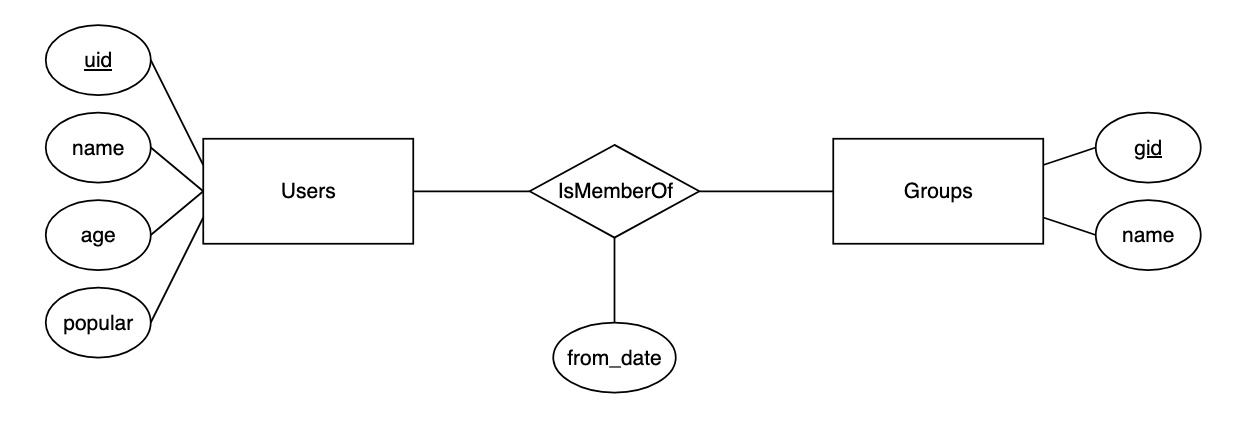
\includegraphics[scale=0.4]{img/social_media.png}
        \caption{Social media database ER diagram.} 
        \label{fig:social_media}
      \end{figure}

      Note that the \texttt{from\_date} attribute must be a part of the Member relation since it isn't uniquely associated with a user (a user can join multiple groups on different dates) or a group (two users can join a group on different dates). If there is an instance that someone joins, leaves, and rejoins a group, then we can modify our design by either: 
      \begin{enumerate}
        \item overwriting the first date joined 
        \item making another relation \texttt{MembershipRecords} which has a date also part of the key, which will capture historical membership.  
      \end{enumerate}
    \end{example}

    Therefore, we must determine if a relation models an entity or a relationship. There could also be multiple relationship sets between the same entity sets, e.g. if \texttt{Member} and \texttt{Likes} associates between \texttt{Users} and \texttt{Groups}. 

\subsection{Relationships and Multiplicity} 

    A relationship really stores minimal information in the sense that if you have you know the entities it connects, that determines everything about the relation. 

    \begin{theorem}[Relationships are Functionally Dependent on Connecting Entities]
      In a relationship set, each relationship is uniquely identified by the entities it connects. More formally, if a relationship $R$ connects entities $e_1 \in E_1, \ldots, e_n \in E_n$ with keys $\mathbf{k} = (k_1, \ldots, k_n)$, then $\mathbf{k}$ is a superkey of $R$. 
    \end{theorem}

  \subsubsection{Multiplicity of Binary Relationships}

    The 4 categories representing the multiplicity just further categorizes how this functional dependency is realized. 

    \begin{definition}[Multiplicity of 2-Way Relationships]
      Given that $E$ and $F$ are entity sets, 
      \begin{enumerate}
        \item \textit{Many-many}: Each entity in E is related to $0$ or more entities in $F$ and vice versa. There are no restrictions, and we have \texttt{IsMemberOf(\underline{uid}, \underline{gid})}.\footnote{Note that this is just a restating of the theorem before.} 

        \begin{figure}[H]
          \centering 
          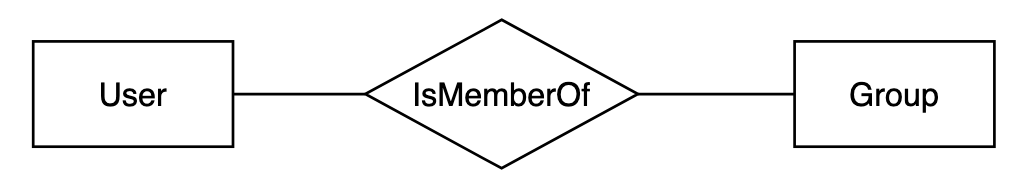
\includegraphics[scale=0.3]{img/ismember.png}
          \caption{} 
          \label{fig:ismember}
        \end{figure}

        \item \textit{Many-One}: Each entity in $E$ is related to $0$ or $1$ entities in $F$, but each entity in $F$ is related to $0$ or more in $E$. If $E$ points to $F$ with a straight arrow, then you can just think that this is a function, and we have \texttt{IsOwnedBy(\underline{gid}, uid)}. If we have a rounded arrow, this means that for each group, its owner \texttt{must} exist in \texttt{Users} (so no $0$). 

        \begin{figure}[H]
          \centering 
          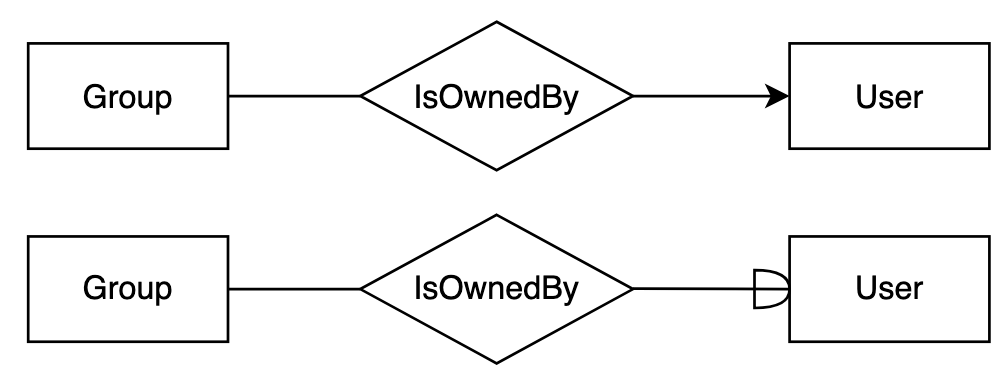
\includegraphics[scale=0.3]{img/isowned.png}
          \caption{} 
          \label{fig:isowned}
        \end{figure}

      \item \textit{One-One}: Each entity in $E$ is related to $0$ or $1$ entity in $F$ and vice versa. We can have either \texttt{IsLinkedTo(\underline{uid}, twitter\_uid)} or \texttt{IsLinkedTo(uid, \underline{twitter\_uid})} and must choose a primary key from these two possible keys.  

      \begin{figure}[H]
        \centering 
        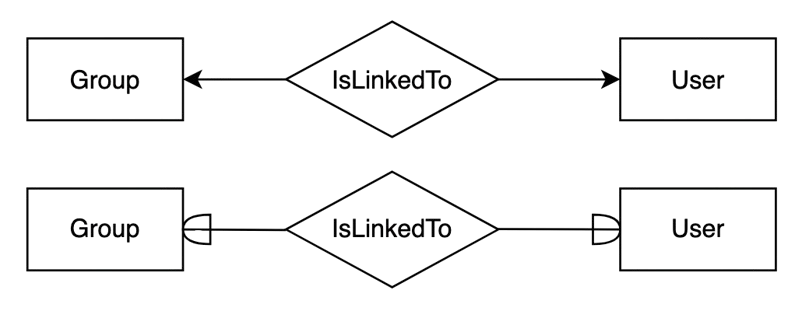
\includegraphics[scale=0.3]{img/islinked.png}
        \caption{} 
        \label{fig:islinked}
      \end{figure}
      \end{enumerate}
    \end{definition}

    \begin{theorem}[Multiplicity with Functional Dependencies]
      You may notice that multiplicity and functional dependence are very similar that is. If we have two relations $R, S$ and have a relationship pointing from $R$ to $S$, then this states the FD $\mathbf{r} \mapsto \mathbf{s}$! Say that the keys are $\mathbf{k}_R, \mathbf{k}_S$, respectively. Then, we have 
      \begin{equation}
        \mathbf{k}_R \mapsto \mathbf{r} \mapsto \mathbf{s} \mapsto \mathbf{k}_S
      \end{equation} 
    \end{theorem}

    \begin{example}[Movie Stars]
      Given the relations 
      \begin{enumerate}
        \item \texttt{Movies(\underline{title, year}, length, name)}
        \item \texttt{Stars(\underline{name}, address)} of a movie star and their address. 
        \item \texttt{Studios(\underline{name}, address)} 
        \item \texttt{StarsIn(\underline{star\_name}, \underline{movie\_name}, \underline{movie\_year})} 
        \item \texttt{Owns(studio\_name, \underline{movie\_name}, \underline{movie\_year})}
      \end{enumerate}
      We have the following ER diagram 
      \begin{figure}[H]
        \centering 
        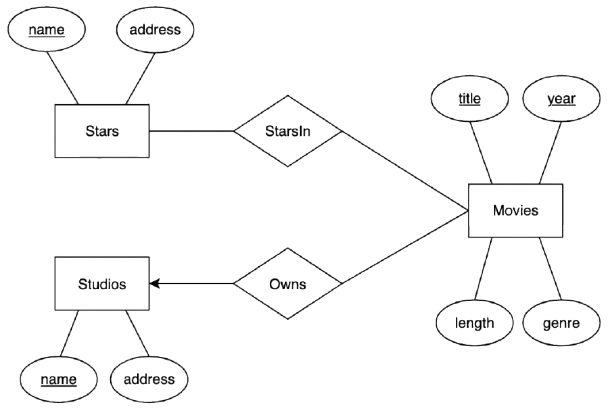
\includegraphics[scale=0.3]{img/movie_stars.png}
        \caption{Movie stars. } 
        \label{fig:movie_stars}
      \end{figure}
    \end{example}

    \begin{example}[Relationship within Itself]
      Sometimes, there is a relationship of an entity set with itself. This gives the relations 
      \begin{enumerate}
        \item \texttt{Users(\underline{uid}, ...)} 
        \item \texttt{IsFriendOf(\underline{uid1}, \underline{uid2})} 
        \item \texttt{IsChildOf(\underline{child\_uid}, parent\_uid)}
      \end{enumerate}
      This can be modeled by the following. Note that 
      \begin{enumerate}
        \item users have no limitations on who is their friend. 
        \item assuming that all parents are single, a person can have at most one parent, so we have an arrow.  
      \end{enumerate}
      \begin{figure}[H]
        \centering 
        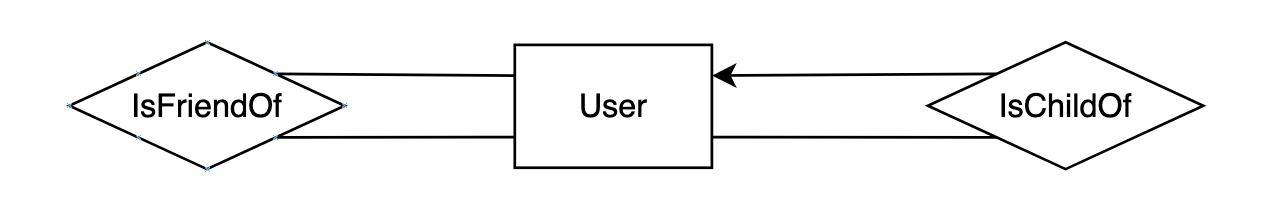
\includegraphics[scale=0.3]{img/within_itself.png}
        \caption{} 
        \label{fig:within_itself}
      \end{figure}
    \end{example}

  \subsubsection{Multiplicity of Multiway Relationships}

    Sometimes, it is necessary to have a relationship between 3 or more entity sets. It can be confusing to contruct the relations with the necessary keys. A general rule of thumb for constructing the relation of a relationship is 
    \begin{enumerate}
      \item Everything that the arrows point into are not keys.   
      \item Everything else are keys. So the arrow stumps are keys. 
    \end{enumerate}

    \begin{example}[Movie Stars]
      Suppose that we wanted to model \textit{Contract} relationship involving a studio, a star, and a movie. This relationships represents that a studio had contracted with a particular star to act in a particular movie. We want a contract to be owned by one studio, but one studio can have multiple contracts for different combinations of stars and movies. This gives the relations 
      \begin{enumerate}
        \item \texttt{Stars(\underline{name}, address)} 
        \item \texttt{Movies(\underline{title, year}, length, name)} 
        \item \texttt{Studios(\underline{name}, address)} 
        \item \texttt{Contracts(\underline{star\_name}, \underline{movie\_name}, studio\_name)}
      \end{enumerate}
      \begin{figure}[H]
        \centering 
        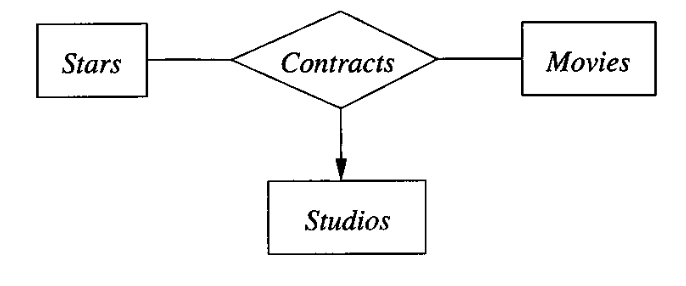
\includegraphics[scale=0.4]{img/contracts.png}
        \caption{} 
        \label{fig:contracts}
      \end{figure}
      We can make this even more complex by modifying contracts to have a studio of the star and the producing studio. 
      \begin{enumerate}
        \item \texttt{Contracts(\underline{star\_name}, \underline{movie\_name}, produce\_studio\_name, star\_studio\_name)}
      \end{enumerate}
      \begin{figure}[H]
        \centering 
        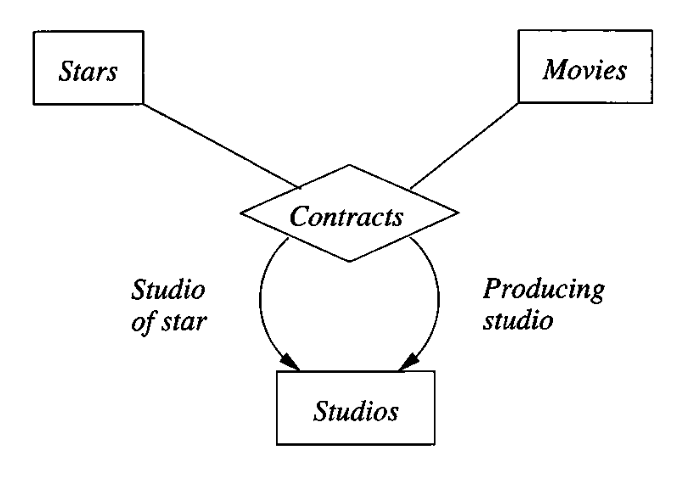
\includegraphics[scale=0.4]{img/four_ary.png}
        \caption{} 
        \label{fig:four_ary}
      \end{figure}
      Note that contracts can also have attributes, e.g. salary or time period. 
    \end{example}

    \begin{example}[Social Media]
      In a 3-ary relationship a user must have an initiator in order to join a group. In here, the \texttt{isMemberOf} relation has an initiator, which must be unique for each initiated member, for a given group. 
      \begin{enumerate}
        \item \texttt{User(\underline{uid}, ...)} 
        \item \texttt{Group(\underline{gid}, ...)} 
        \item \texttt{IsMemberOf(\underline{member}, initiator, \underline{gid})} since a member must have a unique pair of initiator/group that they are in. 
      \end{enumerate}
      \begin{figure}[H]
        \centering 
        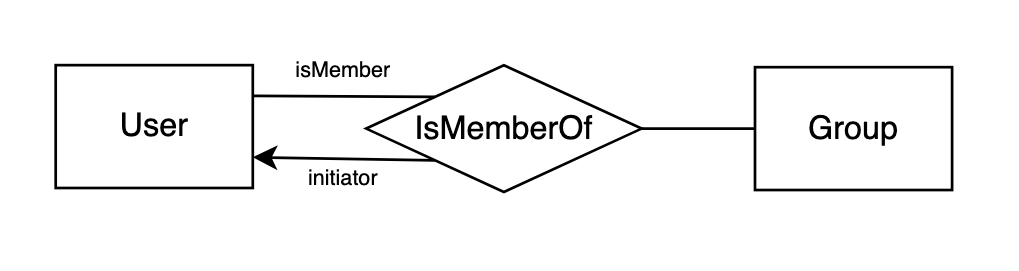
\includegraphics[scale=0.3]{img/three_ary.png}
        \caption{} 
        \label{fig:three_ary}
      \end{figure}
    \end{example}

    But can we model n-ary relationships with only binary relationships? Our intuition says we can't, for the same reasons that we get lossy decomposition into 2-attribute schemas when we try to satisfy BCNF. 

    \begin{example}[N-ary Relationships vs Multiple Binary Relationships]
      N-ary relationships in general cannot be decomposed into multiple binary relationships. Consider the following diagram. 
      \begin{figure}[H]
        \centering 
        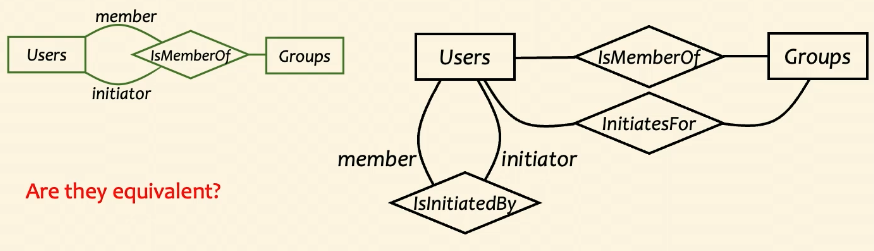
\includegraphics[scale=0.4]{img/nary_vs_binary.png}
        \caption{Attempt at reducing nary to binary ER relationships. } 
        \label{fig:}
      \end{figure}
      \begin{enumerate}
        \item u1 is in both g1 and g2, so \texttt{IsMemberOf} contains both (u1, g1) and (u2, g2)
        \item u2 served as both an initiator in both g1 and g2, so \texttt{InitiatesFor} contains both (g1, u2) and (g2, u2). 
        \item But in reality, u1 was initiated by u2 for g1 but not u2 for g2. This contradicts the information that you would get when joining the \texttt{IsMemberOf} and \texttt{InitiatesFor} relations. 
      \end{enumerate}
      Therefore, combining binary relations may generate something spurious that isn't included in the n-ary relationship. 
    \end{example}

\subsection{Subclasses of Entity Sets}

  Sometimes, an entity set contains certain entities that have special properties not associated with all members of the set. We model this by using a \textbf{isa} relationship with a triangle. 
  
  \begin{figure}[H]
    \centering 
    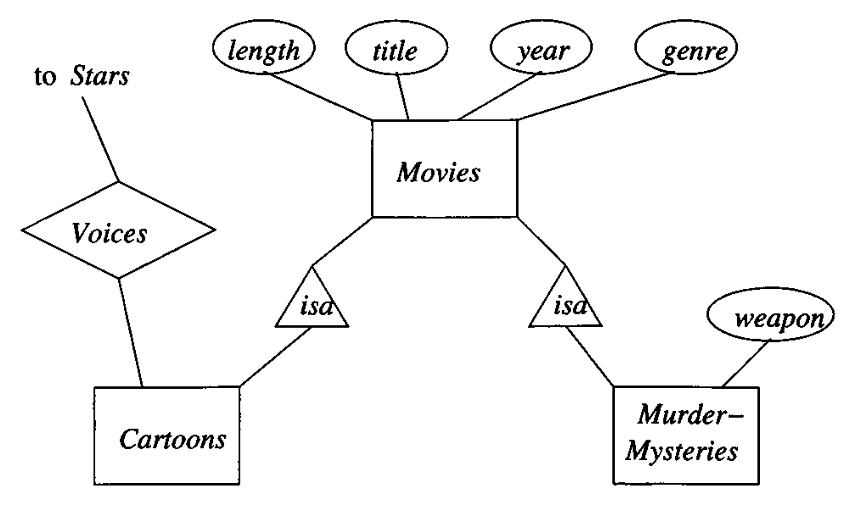
\includegraphics[scale=0.4]{img/isa.png}
    \caption{There are two types of movies: cartoons and murder-mysteries, which can have their own sub-attributes and their own relationships.} 
    \label{fig:isa}
  \end{figure}

  Suppose we have a tree of entity sets, connected by \textit{isa} relationships. A single entity consists of \textit{components} from one or more of these entity sets, and each component is inherited from its parent. 

\subsection{Weak Entity Sets}

  It is possible for an entity set's key to be composed of attributes, some or all of which belong to another entity set. There are two reasons why we need weak entity sets. 
  \begin{enumerate}
    \item Sometimes, entity sets fall into a hierarchy based on classifications unrelated to the \textit{isa} hierarchy. If entities of set $R$ are subunits of entities in set $F$, it is possible that the names of $R$-entities are not unique until we take into account the name of its $S$-entity.\footnote{Think of university rooms in different buildings.}
    \item The second reason is that we want to eliminate multiway relationships, which are not common in practice anyways. These weak entity sets have no attributes and have keys purely from its supporting sets. 
  \end{enumerate}

  \begin{definition}[Weak Entity Set]
    A \textbf{weak entity set} $R$ (double rectangles) depends on other sets. It is an entity set that 
    \begin{enumerate}
      \item has a key consisting of 0 or more of its own attributes, and 
      \item has key attributes from \textbf{supporting entity sets} that are reached by many-one \textbf{supporting relationships} (double diamonds) from it to other sets $S$. 
    \end{enumerate}
    It must satisfy the following. 
    \begin{enumerate}
      \item The relationship $T$ must be binary and many-one from $R$ to $S$. 
      \item $T$ must have referential integrity from $R$ to $S$ (since these are keys and therefore must exist in supporting sets), which is why we have a rounded arrow. 
      \item The attributes that $S$ supplies for the key of $R$ must be key attributes of $S$, unless $S$ is also weak, and it will get keys from its supporting entity set. 
      \item If there are several different supporting relationships from $R$ to the same $S$, then each relationship is used to supply a copy of the key attributes of $S$ to help form the key of $R$. 
    \end{enumerate}
    If an entity set supplies any attributes for its own key, then those attributes will be underlined. 
  \end{definition}

  \begin{example}
    To specify a location, it is not enough to specify just the seat number. The room number, and the building name must be also specified to provide the exact location. There are no extra attributes needed for this subclass, which is why a \textit{isa} relationship doesn't fit into this. 
    \begin{figure}[H]
      \centering 
      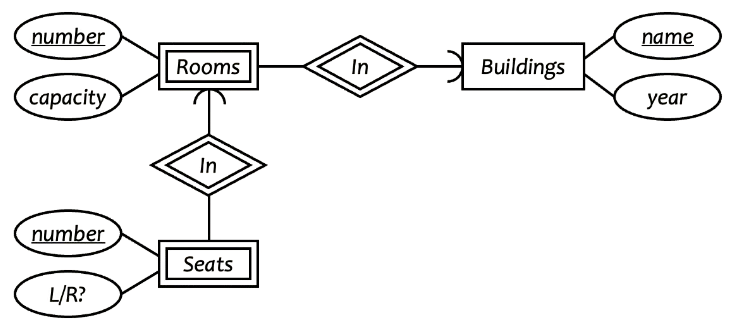
\includegraphics[scale=0.4]{img/weak_entity.png}
      \caption{Specifying a seat is not enough to determine the exact location in a university. We must know the room number and the building to fully identify it. Note that we must keep linking until we get to a regular, non-weak entity. } 
      \label{fig:weak_entity}
    \end{figure}
  \end{example}

  We generally want to use a weak entity set if an entity does not have attributes to define itself. 
  
  \begin{example}
    Say that we want to make a database with the constraints. 
    \begin{enumerate}
      \item For states, record the name and capital city. 
      \item For counties, record the name, area, and location (state) 
      \item For cities, record the name, population, and location (county and state) 
      \item Names of states should be unique. 
      \item Names of counties are unique within a state. 
      \item Names of cities are unique within a county. 
      \item A city is always located in a single county. 
      \item A county is always located in a single state. 
    \end{enumerate}
    Then, our ER diagram may look like 
    \begin{figure}[H]
      \centering 
      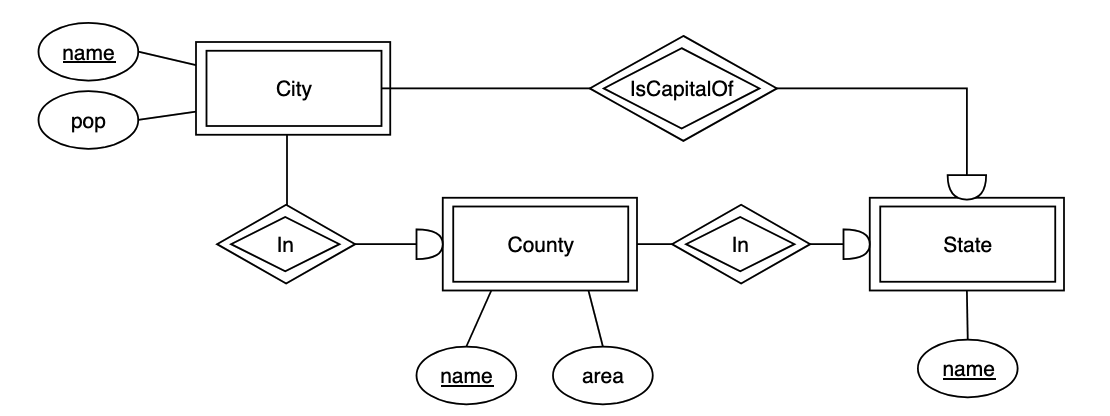
\includegraphics[scale=0.3]{img/city1.png}
      \caption{A weakness is that this doesn't prevent a city in state $X$ from being the capital of another state $Y$.} 
      \label{fig:city1}
    \end{figure}
  \end{example}

  \begin{example}
    Design a database with the following. 
    \begin{enumerate}
      \item A station has a unique name and address, and is either an express station or a local station. 
      \item A train has a unique number and engineer, and is either an express or local train. 
      \item A local train can stop at any station. 
      \item An express train only stops at express stations. 
      \item A train can stop at a station for any number of times during a train. 
      \item Train schedules are the same every day. 
    \end{enumerate}
    Then, our ER diagram may look like 
    \begin{figure}[H]
      \centering 
      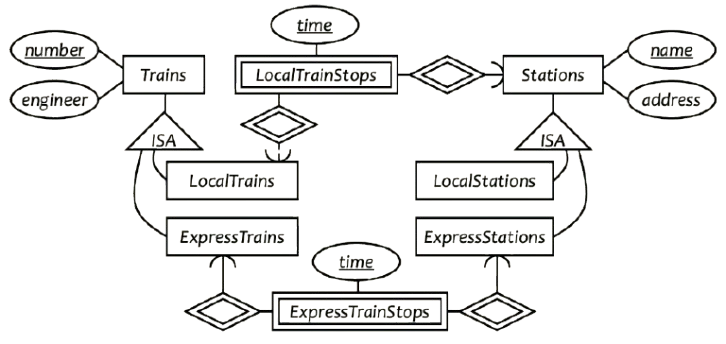
\includegraphics[scale=0.4]{img/train1.png}
      \caption{} 
      \label{fig:train1}
    \end{figure}
  \end{example}

\subsection{Translating ER Diagrams to Relational Designs}

  One a simple level, converting an ER diagram to a relational database schema is straightforward. Here are some rules we list. 

  \begin{theorem}[Converting Entity Sets]
    Turn each entity set into a relation with the same set of attributes. 
  \end{theorem}

  \begin{theorem}[Converting Relationships]
    Replace a relationship by a relation whose attributes are the keys for the connected entity sets along with its own attributes. If an entity set is involved several times in a relationship, then its key attributes are repeated, so you must rename them to avoid duplication.
  \end{theorem}

  \begin{theorem}[Reduce Repetition for Many-One Relationships]
    We can actually reduce repetition for many-one relationships. For example, if there is a many-one relationship $T$ from relation $R$ to relation $S$, then $\mathbf{r}$ functionally determines $\mathbf{s}$, so we can combine them into one relation consisting of 
    \begin{enumerate}
      \item all attributes of $R$. 
      \item key attributes of $S$. 
      \item Any attributes belonging to relationship $T$. 
    \end{enumerate}
  \end{theorem}
  
  \begin{theorem}[Handling Weak Entity Sets]
    To build weak entity sets, we must do three things. 
    \begin{enumerate}
      \item The relation for weak entity set $W$ must include its own attributes, all key (but not non-key) attributes of supporting entity sets, and all attributes for supporting relationships for $W$. 
      \item The relation for any relationship where $W$ appears must use the entire set of keys gotten from $W$ and its supporting entity sets. 
      \item Supporting relationships should not be converted since they are many-one, so we can use the reduce repetition for many-one relationships rule above. 
    \end{enumerate}
  \end{theorem}

  \begin{example}
    To translate the seat, rooms, and buildings diagram, 
    \begin{figure}[H]
      \centering 
      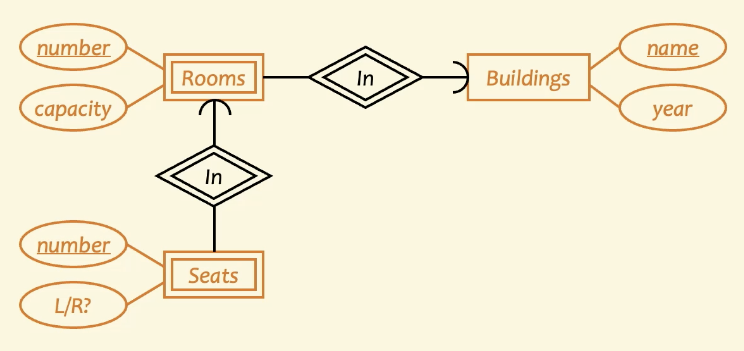
\includegraphics[scale=0.4]{img/seat.png}
      \caption{} 
      \label{fig:seat}
    \end{figure}
    we have 
    \begin{enumerate}
      \item \texttt{Building(\underline{name}, year)} 
      \item \texttt{Room(\underline{building\_name}, \underline{room\_num}, capacity)}
      \item \texttt{Seat(\underline{building\_name}, \underline{room\_num}, \underline{seat\_num}, left\_or\_right)}
    \end{enumerate}
    Note that we do not need to convert the relationships since they are contained within the entity set relations. So ignore double diamonds. 
  \end{example}

  \begin{figure}[H]
    \centering 
    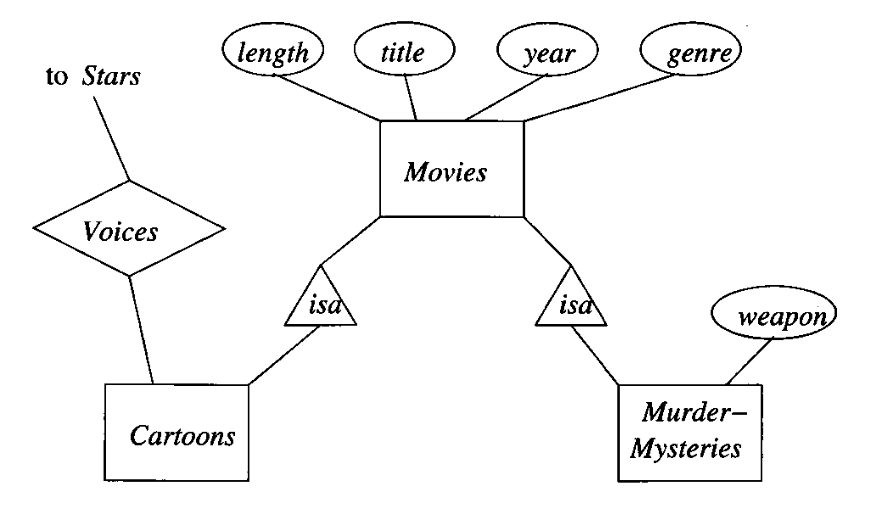
\includegraphics[scale=0.45]{img/movie_hierarchy.png}
    \caption{A figure of the movie hierarchy for convenience. } 
    \label{fig:movie_hierarchy}
  \end{figure}

  \begin{theorem}[Converting Subclass Structures]
    To convert subclass structure with a \textit{isa} hierarchy, there are multiple ways we can convert them. 
    \begin{enumerate}
      \item \textit{E/R Standard}. An entity is in all superclasses and only contains the attributes its own subclass. For each entity set $R$ in the hierarchy, create a relation that includes the key attributes from the root and any attributes belonging to $R$. This gives us 
        \begin{enumerate}
          \item \texttt{Movies(title, year, length, genre)}
          \item \texttt{MurderMysteries(title, year, weapon)}
          \item \texttt{Cartoons(title, year)}
        \end{enumerate}
      \item \textit{Object Oriented}. For each possible subtree that includes the root, create one relation whose schema includes all the attributes of all entity sets in the subtree.
        \begin{enumerate}
          \item \texttt{Movies(title, year, length, genre)} 
          \item \texttt{MoviesC(title, year, length, genre)} 
          \item \texttt{MoviesMM(title, year, length, genre, weapon)}
          \item \texttt{MoviesCMM(title, year, length, genre, weapon)}
        \end{enumerate}
        Additionally, the relationship would be \texttt{Voices(title, year, starName)}. 
      \item \textit{Null Values}. Create one relation for the entire hierarchy containing all attributes of all entity sets. Each entity is one tuple, and the tuple has null values for attributes the entity does not have. We would in here always have a single schema. 
        \begin{enumerate}
          \item \texttt{Movie(title, year, length, genre, weapon)}
        \end{enumerate}
    \end{enumerate}
  \end{theorem}

  Note that the difference between the first two is that in ER, \texttt{MurderMysteries} does not contain the attributes of its superclass, while in OO, it does. 

  As you probably notice, each standard has pros and cons. The nulls approach uses only one relation, which is simple and nice. To filter out over all movies, E/R is nice since we only filter through \texttt{Movies}, whilst in OO we have to go through all relations. However, when we want to filter movies that are both Cartoons and Murder Mysteries, then OO is better since we can only select from \texttt{MoviesCMM} rather than having to go through multiple relations for ER or filter out with further selections in Null. Also, OO uses the least memory, since it doesn't waste space on null values on attributes.  


  \begin{example}
    Let's put this all together to revisit the train station example. 
    \begin{figure}[H]
      \centering 
      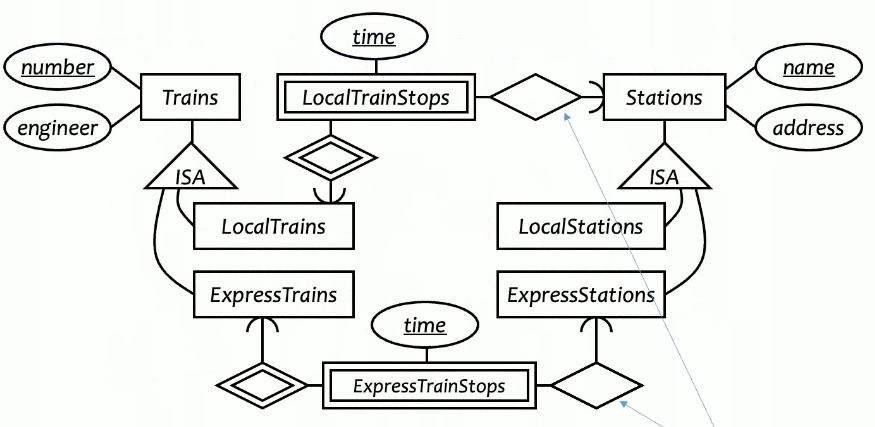
\includegraphics[scale=0.4]{img/final_station.png}
      \caption{For convenience} 
      \label{fig:final_station}
    \end{figure}
    We can use the ER standard to define the first 6 regular relations in single rectangles.  
    \begin{enumerate}
      \item \texttt{Train(\underline{number}, engineer)}
      \item \texttt{LocalTrain(\underline{number}}
      \item \texttt{ExpressTrain(\underline{number}}
      \item \texttt{Station(\underline{name}, address)}
      \item \texttt{LocalStation(\underline{name})}
      \item \texttt{ExpressStation(\underline{name})}
    \end{enumerate}
    Then we can construct the weak entity sets. 
    \begin{enumerate}
      \item \texttt{LocalTrainStops(\underline{local\_train\_num}, \underline{time})}
      \item \texttt{ExpressTrainStops(\underline{express\_train\_num}, \underline{time})}
    \end{enumerate}
    Then we can construct the relationships (marked with the arrows).  
    \begin{enumerate}
      \item \texttt{LocalTrainStopsAtStation(\underline{local\_train\_number}, \underline{time}, station\_name)}
      \item \texttt{ExpressTrainStopsAtStation(\underline{express\_train\_number}, \underline{time}, express\_station\_name)}
    \end{enumerate}
    Note that we can simplify these 10 relations to 8. For example, the \texttt{LocalTrain} and \texttt{LocalStation} relations are redundant since it can be computed as 
    \begin{align}
      LocalTrain & = \pi_{number} (Train) - ExpressTrain \\
      LocalStation & = \pi_{number} (Station) - ExpressStation
    \end{align}
    There is a tradeoff since it's an extra computation when checking. However, if we had used the Null Value strategy, this would be a lot simpler, and we can use value constraints on the train and station type, which can be implemented in the DBMS (though not directly in the ER diagram). 
  \end{example}

